

\documentclass[letter, 10pt, margins=0.3in]{texMemo}

\usepackage{amsmath}
\usepackage{booktabs}
\usepackage{color, soul}
\usepackage{dcolumn}
\usepackage{enumitem}

    \newcolumntype{d}[1]{D{.}{.}{#1}}
\usepackage[colorlinks=true, citecolor=blue]{hyperref}

\usepackage{graphicx, lipsum}

\usepackage{imakeidx}

\usepackage{caption}
\usepackage{subcaption}

\usepackage[LGRgreek]{mathastext}

\usepackage{listings}
\usepackage[]{matlab-prettifier}

\usepackage{multirow}

\usepackage{natbib}
\bibliographystyle{apalike}

\usepackage{printlen}  % \printlength\textwidth - To determine textwidth of document.  Here is it 496 pt.

\usepackage{siunitx}

\usepackage{tablefootnote}

\usepackage[table]{xcolor}
\definecolor{maroon}{cmyk}{0,0.87,0.68,0.32}
\definecolor{LightCyan}{rgb}{0.88,1,1}
\definecolor{Gray}{gray}{0.85}


\newcommand{\is}[1]{%
\if@noftnote%
\index{#1}%
\else%
\index{#1|fn{\number\value{footnote}}}%
\fi%
}

\makeindex


\graphicspath{ {../} }


\memodate{\today~(Submitted)}
\memosubject{ACS 547, Module 4 Assignment - Sound Sources\\}



\begin{document}

\maketitle


\vspace{-1.0cm}
\section*{Problem 1 - Simulation of Sources from Monopoles}


\vspace{-0.25cm}
The Matlab code for this problem is listed in Appendix~\ref{appendix:problem1}.


\vspace{-0.25cm}
\subsection*{Problem 1a}

\vspace{-0.3cm}
Figure~\ref{figure:1aMonopoleSphericalSpreading} shows the spherical spreading from a monopole.  The frequency is 1 kHz.  The sound pressure level has been calculated at two distances:  1 $m$ and 4 $m$.

\vspace{-0.25cm}
\begin{figure}[htb!]
    \center
        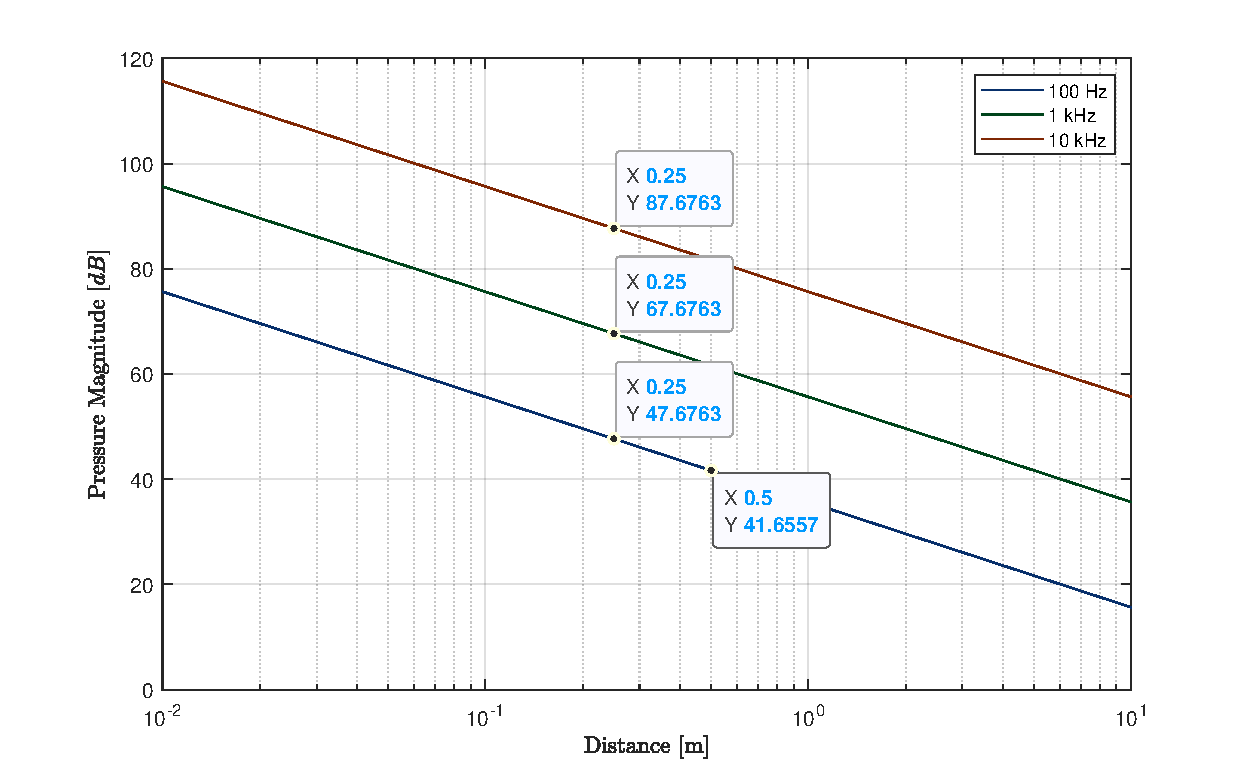
\includegraphics[scale = 0.625, keepaspectratio]{Homework_4_Part_1a.pdf}
    \caption{Monopole spherical spreading for 1 kHz.  The radius of the polar plot is the sound pressure level.}
    \label{figure:1aMonopoleSphericalSpreading}
\end{figure}



Figure~\ref{figure:1aMonopolePressureDrop} shows the sound pressure level as a function of distance for a 1 kHz monopole source.

\vspace{-0.25cm}
\begin{figure}[htb!]
    \center
        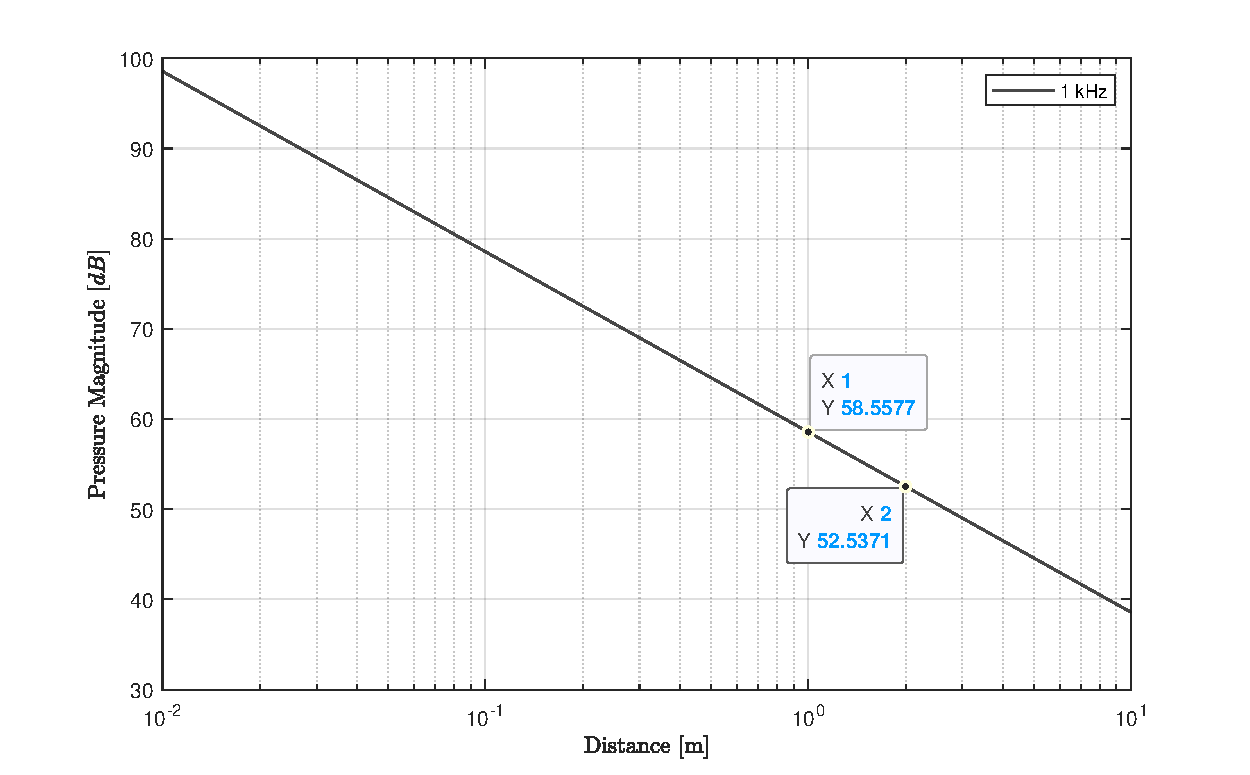
\includegraphics[scale = 0.625, keepaspectratio]{Homework_4_Part_1a2.pdf}
    \caption{Monopole pressure drop versus distance for 1 kHz.}
    \label{figure:1aMonopolePressureDrop}
\end{figure}

The pressure drop is proportional to $\frac{1}{r}$;  doubling the distance yields -6 dB of level change (see data points).





\newpage
\subsection*{Problem 1b}

\vspace{-0.25cm}
Figure~\ref{figure:1bDirectivityPatterns} illustrates the directivity patterns for a monopole, dipole, lateral quadrupole, and a linear quadrupole for 1 kHz.  The receivers were placed at a 1 $m$ distance around each of the sources.

\vspace{-0.3cm}
\begin{figure}[htb!]
    \center
        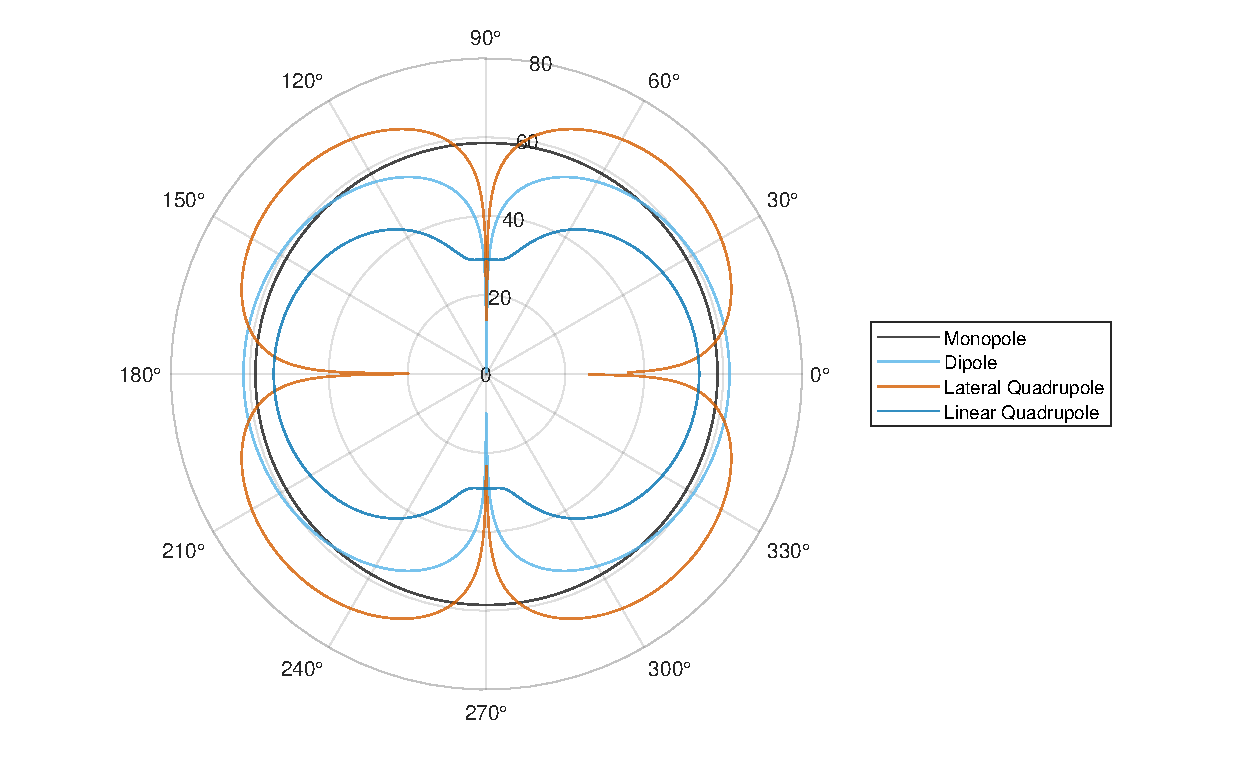
\includegraphics[scale = 0.625, keepaspectratio]{Homework_4_Part_1b.pdf}
    \caption{Directivity patterns for a 1 kHz monopole, dipole, lateral quadrupole, and linear quadrupole.}
    \label{figure:1bDirectivityPatterns}
\end{figure}



\vspace{0.2cm}
Table~\ref{table:1bLevels} lists the sound pressure levels for the 4 types of patterns for 1 kHz.

\vspace{0.25cm}
\setlength{\abovecaptionskip}{1.5pt}
\vspace{0.1cm}
{\renewcommand{\arraystretch}{1.5}
\begin{table}[htpb!]
    \footnotesize
    \centering
        \begin{tabular}{ | c | c | }
        \hline
        \textbf{Source Type}  &  \textbf{Sound Pressure Level [dB]}   \\
        \hline
        Monopole  &  58.6   \\
        \hline
        Dipole  &  61.6   \\
        \hline
        Lateral Quadrupole  &  48.2   \\
        \hline
        Linear Quadrupole  &  53.9  \\
        \hline
        \end{tabular}

        \vspace{0.5cm}
        \caption{Sound pressure levels for 1 kHz at 1 m distance.}
        \label{table:1bLevels}

\end{table}


\vspace{0.25cm}
The monopole had a volume velocity of 1.4 $\frac{m^3}{s}$.

\vspace{0.25cm}
The dipole had two equal strength, in-phase elements with a separation of 0.0429 $m$, which is less than the 1 $kHz$ wavelength of 0.343 $m$.  The volume velocity for both sources was 1.4 $\frac{m^3}{s}$.

\vspace{0.25cm}
The lateral quadrupole had four equal strength, diagonally opposite in-phase pairs with a separation of 0.0429 $m$.  The volume velocity for both sources was 1.4 $\frac{m^3}{s}$.

\vspace{0.25cm}
The linear quadrupole had three sources, the end sources were equal strength and in-phase, while the center source was twice the strength of the single sources and 180 $^\circ$ out-of-phase.  The separation between all three sources was 0.0429 $m$.  The volume velocity of the end sources was 1.4 $\frac{m^3}{s}$ and the volume velocity for the center source was 2.8 $\frac{m^3}{s}$.





\newpage
\subsection*{Problem 1c}

Figure~\ref{figure:1cLineSourceSmallSeparation} shows a set of directivity patterns for a 9-element line source with a separated of 0.0429 $m$ centered at the origin along the x-axis (demarcated by the 180$^\circ$ to 0$^\circ$ line in the polar plot) for 100 Hz, 2 kHz, and 5 kHz.  The receivers are placed at a 1 $m$ distance around the line source.

\begin{figure}[htb!]
    \center
        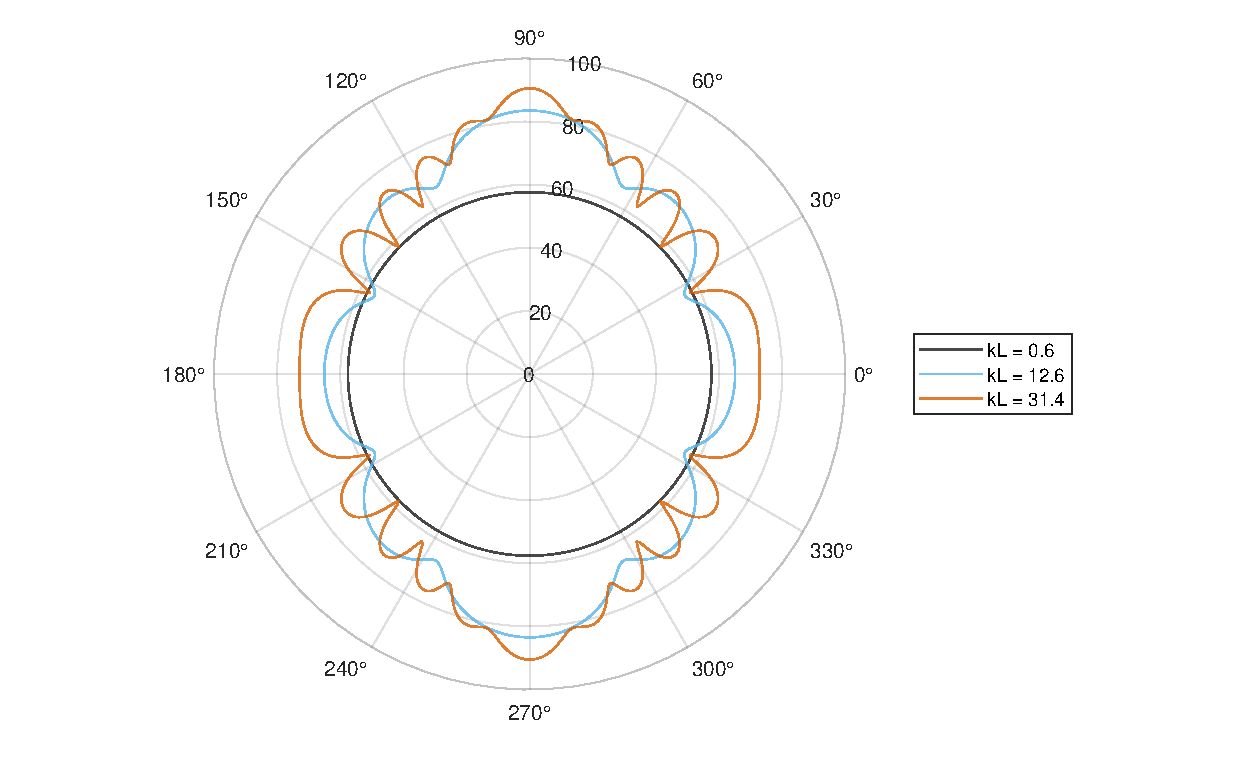
\includegraphics[scale = 0.68, keepaspectratio]{Homework_4_Part_1c.pdf}
    \caption{Line source directivity patterns for frequencies of 100 Hz, 2 kHz, and 5 kHz with small source separation.}
    \label{figure:1cLineSourceSmallSeparation}
\end{figure}

\vspace{0.25cm}
The length of the array is 0.343 $m$, or the 1 kHz wavelength.  As the frequency of the source increases (i.e., $k\cdot L$), the patterns have larger directivity but with more side lobes.


\vspace{0.25cm}
Figure~\ref{figure:1cLineSourceLargeSeparation} shows the directivity patterns for a similar line source, but with the sources now separated by 0.172 $m$.

\begin{figure}[htb!]
    \center
        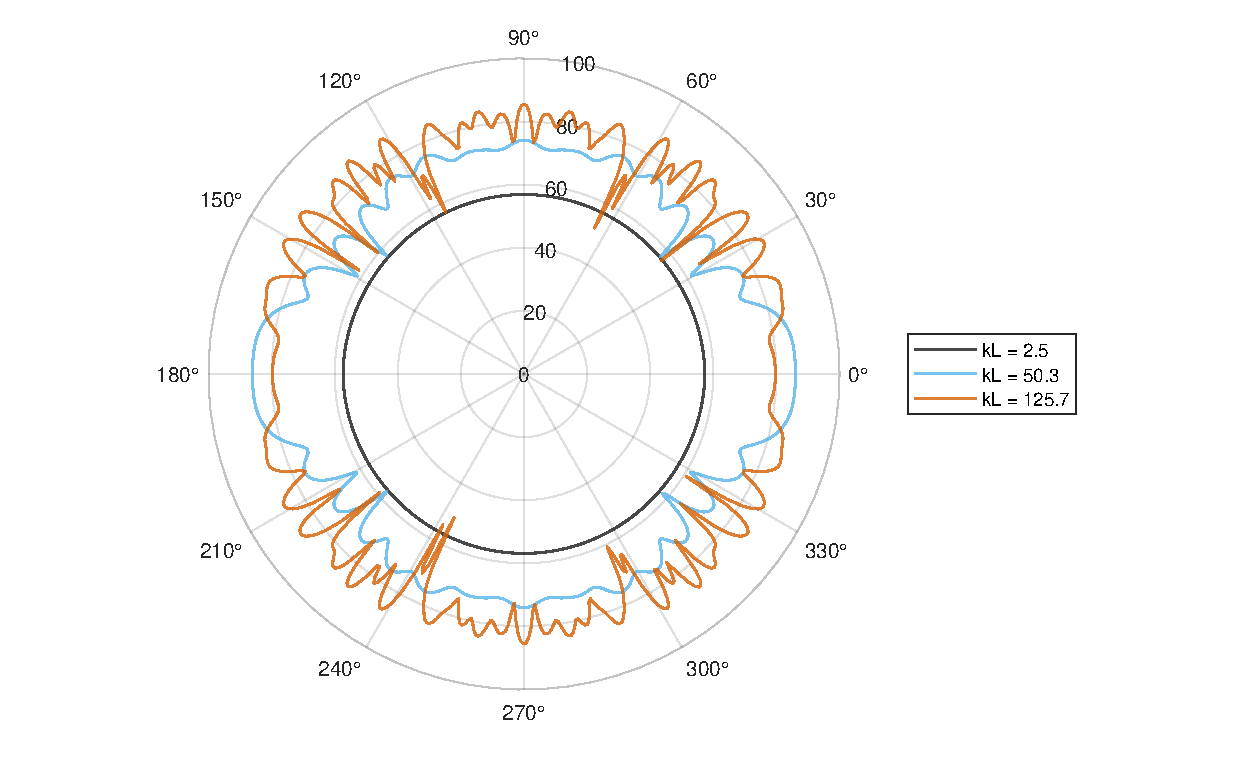
\includegraphics[scale = 0.675, keepaspectratio]{Homework_4_Part_1c2.pdf}        
    \caption{Line source directivity patterns for frequencies of 100 Hz, 2 kHz, and 5 kHz with large source separation.}
    \label{figure:1cLineSourceLargeSeparation}
\end{figure}

\vspace{0.25cm}
The length of the array is now 1.37 $m$, or 4 times the 1 kHz wavelength.  As the frequency of the source increases (i.e., $k\cdot L$), the patterns have larger directivity but with more side lobes.  Here, unlike the previous case, there are a greater number of side lobes for the 2 kHz signal (blue curve).





\newpage
\subsection*{Problem 1d}

Figure~\ref{figure:1dBaffledPistonSourceLocations} shows the monopole source locations in the xy-plane.  The number of sources in the plane was 100 and ``$a$'' was set to 1.715 $m$ (5 times the 1 kHz wavelength of 0.343 $m$).

\begin{figure}[htb!]
    \center
        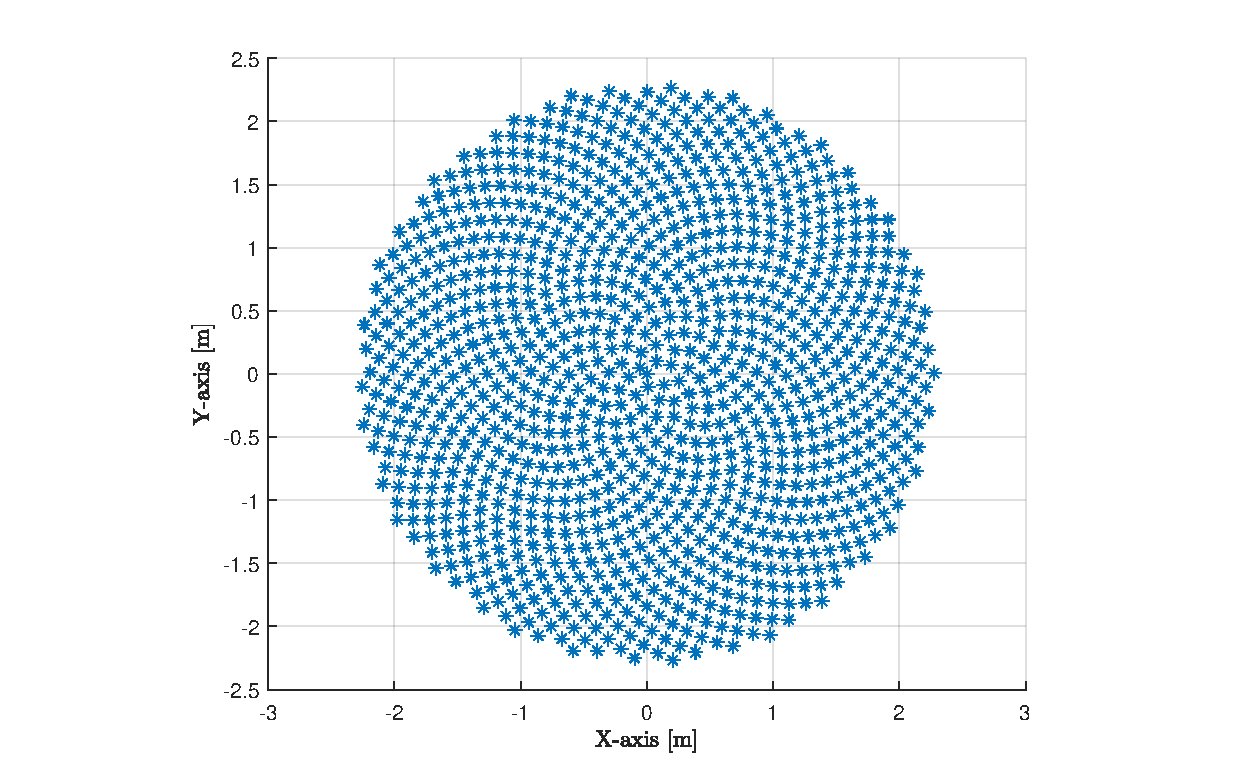
\includegraphics[scale = 0.675, keepaspectratio]{Homework_4_Part_1d.pdf}
    \caption{Monopole source locations in the xy-plane.}
    \label{figure:1dBaffledPistonSourceLocations}
\end{figure}



\vspace{0.35cm}
Figure~\ref{figure:1dBaffledPistonDirectivity} shows the estimated and theoretical null locations along the z-axis above the xy-place for the baffled piston.

\begin{figure}[htb!]
    \center
        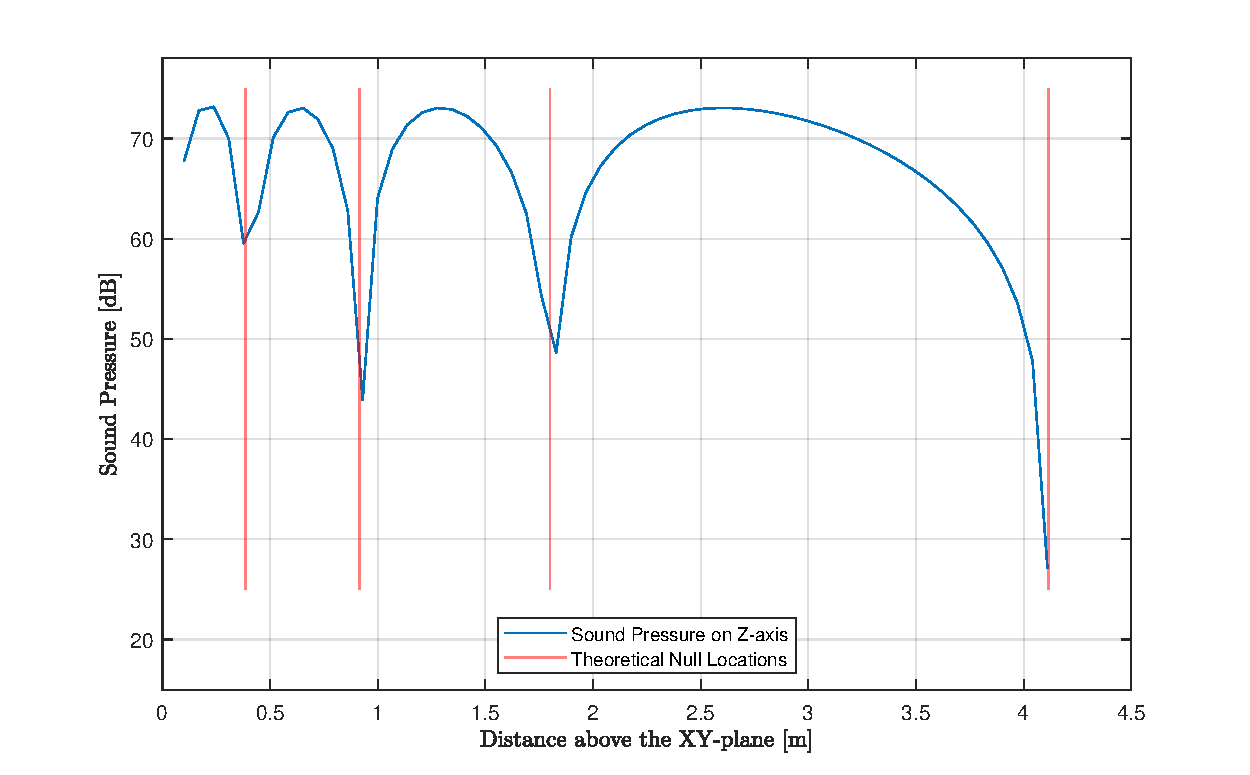
\includegraphics[scale = 0.675, keepaspectratio]{Homework_4_Part_1d2.pdf}
    \caption{The estimated and theoretical null locations along the z-axis for the baffled piston.}
    \label{figure:1dBaffledPistonDirectivity}
\end{figure}

\vspace{0.25cm}
The factor $\frac{a}{\lambda}$ was 5;  there are 5 theoretical null locations.  There is good agreement between the estimated and theoretical null points.  The estimated null near the surface of the piston is governed by starting receiver location on the z-axis.  As this distance is made smaller, the sound pressure level grows rapidly due to the calculation method of the monopole sources.





\newpage
\section*{Problem 2 - Active Control of Enclosure Opening}
\setcounter{figure}{0}
\setcounter{table}{0}
\setcounter{footnote}{0}


The Matlab code for this problem is listed in Appendix~\ref{appendix:problem2}.


\subsection*{Problem 2a}

Figure~\ref{figure:2aSoundPowerLevelReduction} shows the sound pressure level reduction versus octave band frequency for the linear quadrupole.

\vspace{-0.25cm}
\begin{figure}[htb!]
    \center
        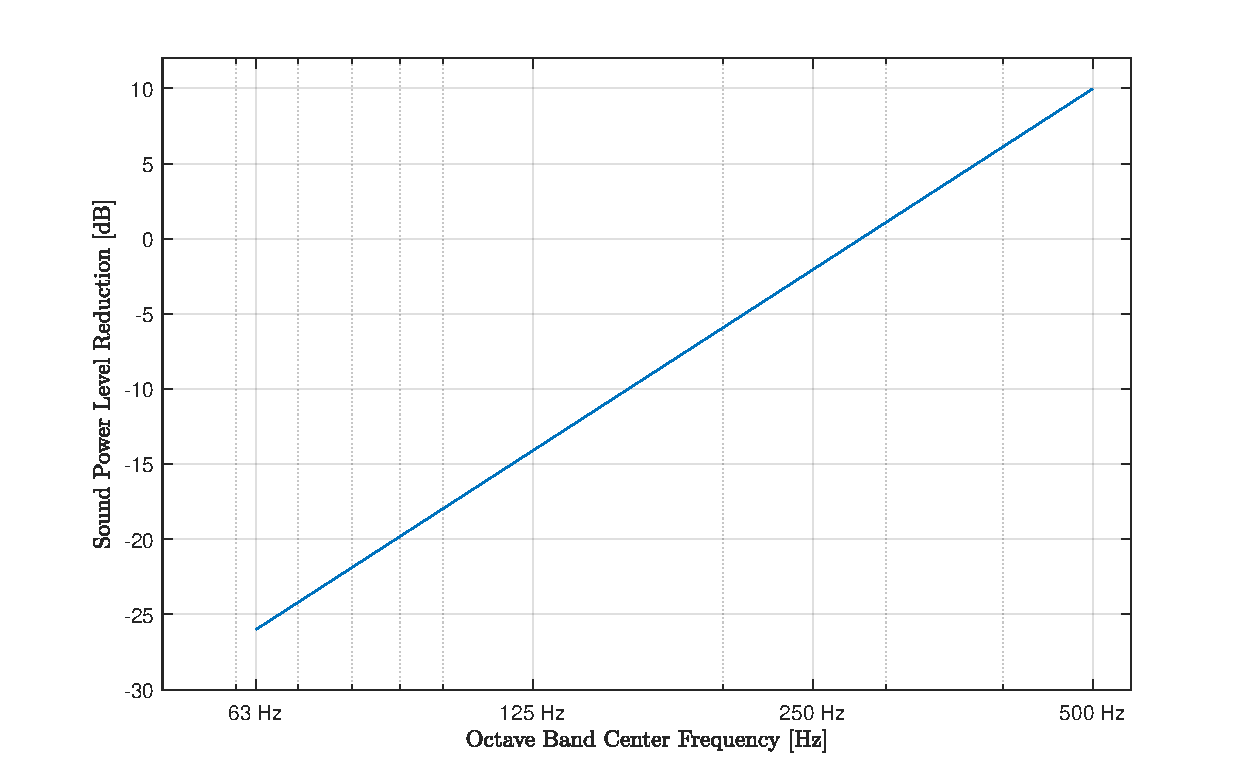
\includegraphics[scale = 0.675, keepaspectratio, trim=4 4 4 4, clip]{Homework_4_Part_2a.pdf}
    \caption{Sound pressure level reduction as a function of octave band center frequency.}
    \label{figure:2aSoundPowerLevelReduction}
\end{figure}


%\vspace{0.2cm}
%Table~\ref{table:2aLevels} lists the sound power level reduction for the 63, 125, 250, and 500 Hz octave bands.
%
%\vspace{0.25cm}
%\setlength{\abovecaptionskip}{1.5pt}
%\vspace{0.1cm}
%{\renewcommand{\arraystretch}{1.5}
%\begin{table}[htpb!]
%    \footnotesize
%    \centering
%        \begin{tabular}{ | c | c | }
%        \hline
%        \textbf{Octave Band [Hz]}  &  \textbf{Level Reduction [dB]}   \\
%        \hline
%        63  &  -26.0   \\
%        \hline
%        125  &  -14.1   \\
%        \hline
%        250  &  -2.1   \\
%        \hline
%        500  &  10.0  \\
%        \hline
%        \end{tabular}
%
%        \vspace{0.5cm}
%        \caption{Octave band sound power level reductions.}
%        \label{table:2aLevels}
%
%\end{table}




\vspace{-0.25cm}
\subsection*{Problem 2b}

Figure~\ref{figure:2aSoundPowerLevelReductionVersusTheta} shows the octave sound level reduction versus the angle, $\theta$, between the plane of the opening and a line at the center of the box opening.

\vspace{-0.25cm}
\begin{figure}[htb!]
    \center
        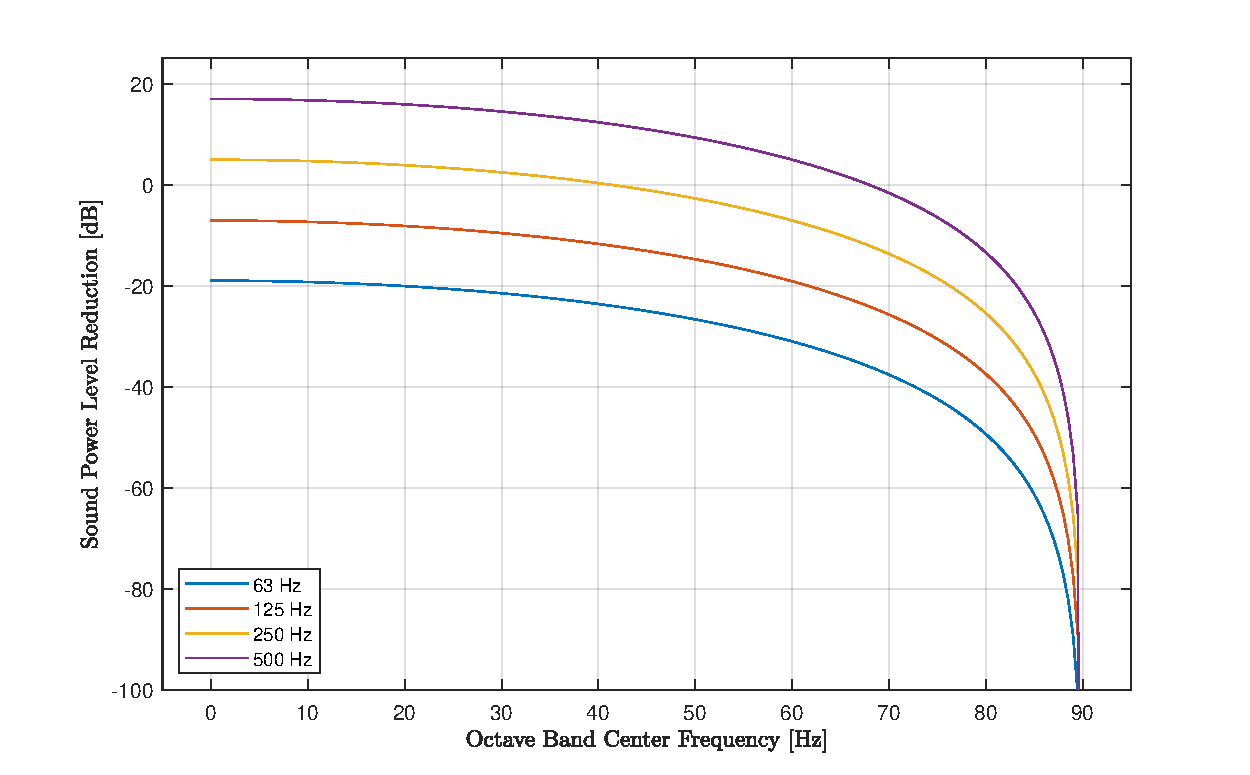
\includegraphics[scale = 0.675, keepaspectratio, trim=4 4 4 4, clip]{Homework_4_Part_2b.pdf}
    \caption{Octave band pressure level reduction as a function theta.}
    \label{figure:2aSoundPowerLevelReductionVersusTheta}
\end{figure}


\vspace{0.25cm}
The relative level reduction across the four octave bands is similar.  As the receiver moves from the side of the opening towards its center, the level of reduction increases, where at 90$^\circ$, a null is reached as shown in Figure~\ref{figure:1bDirectivityPatterns} for Problem 1b.







\section*{Problem 3 - Coherent and Incoherent Speakers}
\setcounter{figure}{0}
\setcounter{table}{0}
\setcounter{footnote}{0}


The Matlab code for this problem is listed in Appendix~\ref{appendix:problem3}.


\subsection*{Part 3a}

The expected sound pressure at the receive for the coherent sources is -17.3 dB.


\subsection*{Part 3b}

The expected sound pressure at the receive for the incoherent sources is -17.3 dB.







\newpage
\section*{Problem 4 - Washing Machine Abuse Testing}
\setcounter{figure}{0}
\setcounter{table}{0}
\setcounter{footnote}{0}


The Matlab code for this problem is listed in Appendix~\ref{appendix:problem4}.


\subsection*{Part 4a}










\newpage
\section{Appendix - Matlab Code for Problem 1}
\label{appendix:problem1}

\lstinputlisting[style=Matlab-editor, numbers=left, mlshowsectionrules, basicstyle=\scriptsize]{../ACS_547_Module_4_Question_1_Monday_March_31_2025.m}


\newpage
\section{Appendix - Matlab Code for Problem 2}
\label{appendix:problem2}

\lstinputlisting[style=Matlab-editor, numbers=left, mlshowsectionrules, basicstyle=\scriptsize]{../ACS_547_Module_4_Question_2_Monday_March_31_2025.m}


\newpage
\section{Appendix - Matlab Code for Problem 3}
\label{appendix:problem3}

\lstinputlisting[style=Matlab-editor, numbers=left, mlshowsectionrules, basicstyle=\scriptsize]{../ACS_547_Module_4_Question_3_Monday_March_31_2025.m}


\newpage
\section{Appendix - Matlab Code for Problem 4}
\label{appendix:problem4}

\lstinputlisting[style=Matlab-editor, numbers=left, mlshowsectionrules, basicstyle=\scriptsize]{../ACS_547_Module_4_Question_4_Monday_March_31_2025.m}






\end{document}


% Reference(s):

% https://tex.stackexchange.com/questions/180222/how-to-change-font-size-for-specific-lstlisting









